% Source - https://tex.stackexchange.com/a/344324
% Posted by JiyuuSensei, modified by community. See post 'Timeline' for change history
% Retrieved 2026-02-05, License - CC BY-SA 3.0

\documentclass{standalone}
\usepackage{pgfgantt}

% Custom bar styles (these DO NOT create new commands; they create styles)
\newganttchartelement{orangebar}{
  orangebar/.style={
    inner sep=0pt,
    draw=red!66!black,
    very thick,
    top color=white,
    bottom color=orange!80
  },
  orangebar label font=\slshape,
  orangebar left shift=.1,
  orangebar right shift=-.1
}

\newganttchartelement{bluebar}{
  bluebar/.style={
    inner sep=0pt,
    draw=purple!44!black,
    very thick,
    top color=white,
    bottom color=blue!80
  },
  bluebar label font=\slshape,
  bluebar left shift=.1,
  bluebar right shift=-.1
}

\newganttchartelement{greenbar}{
  greenbar/.style={
    inner sep=0pt,
    draw=green!50!black,
    very thick,
    top color=white,
    bottom color=green!80
  },
  greenbar label font=\slshape,
  greenbar left shift=.1,
  greenbar right shift=-.1
}

\newganttchartelement{redbar}{
  redbar/.style={
    inner sep=0pt,
    draw=red!66!black,
    very thick,
    top color=white,
    bottom color=red!80
  },
  redbar label font=\slshape,
  redbar left shift=.1,
  redbar right shift=-.1
}

\newganttchartelement{blackbar}{
  blackbar/.style={
    inner sep=0pt,
    draw=black,
    very thick,
    top color=white,
    bottom color=black
  },
  blackbar label font=\slshape,
  blackbar left shift=.1,
  blackbar right shift=-.1
}


\begin{document}
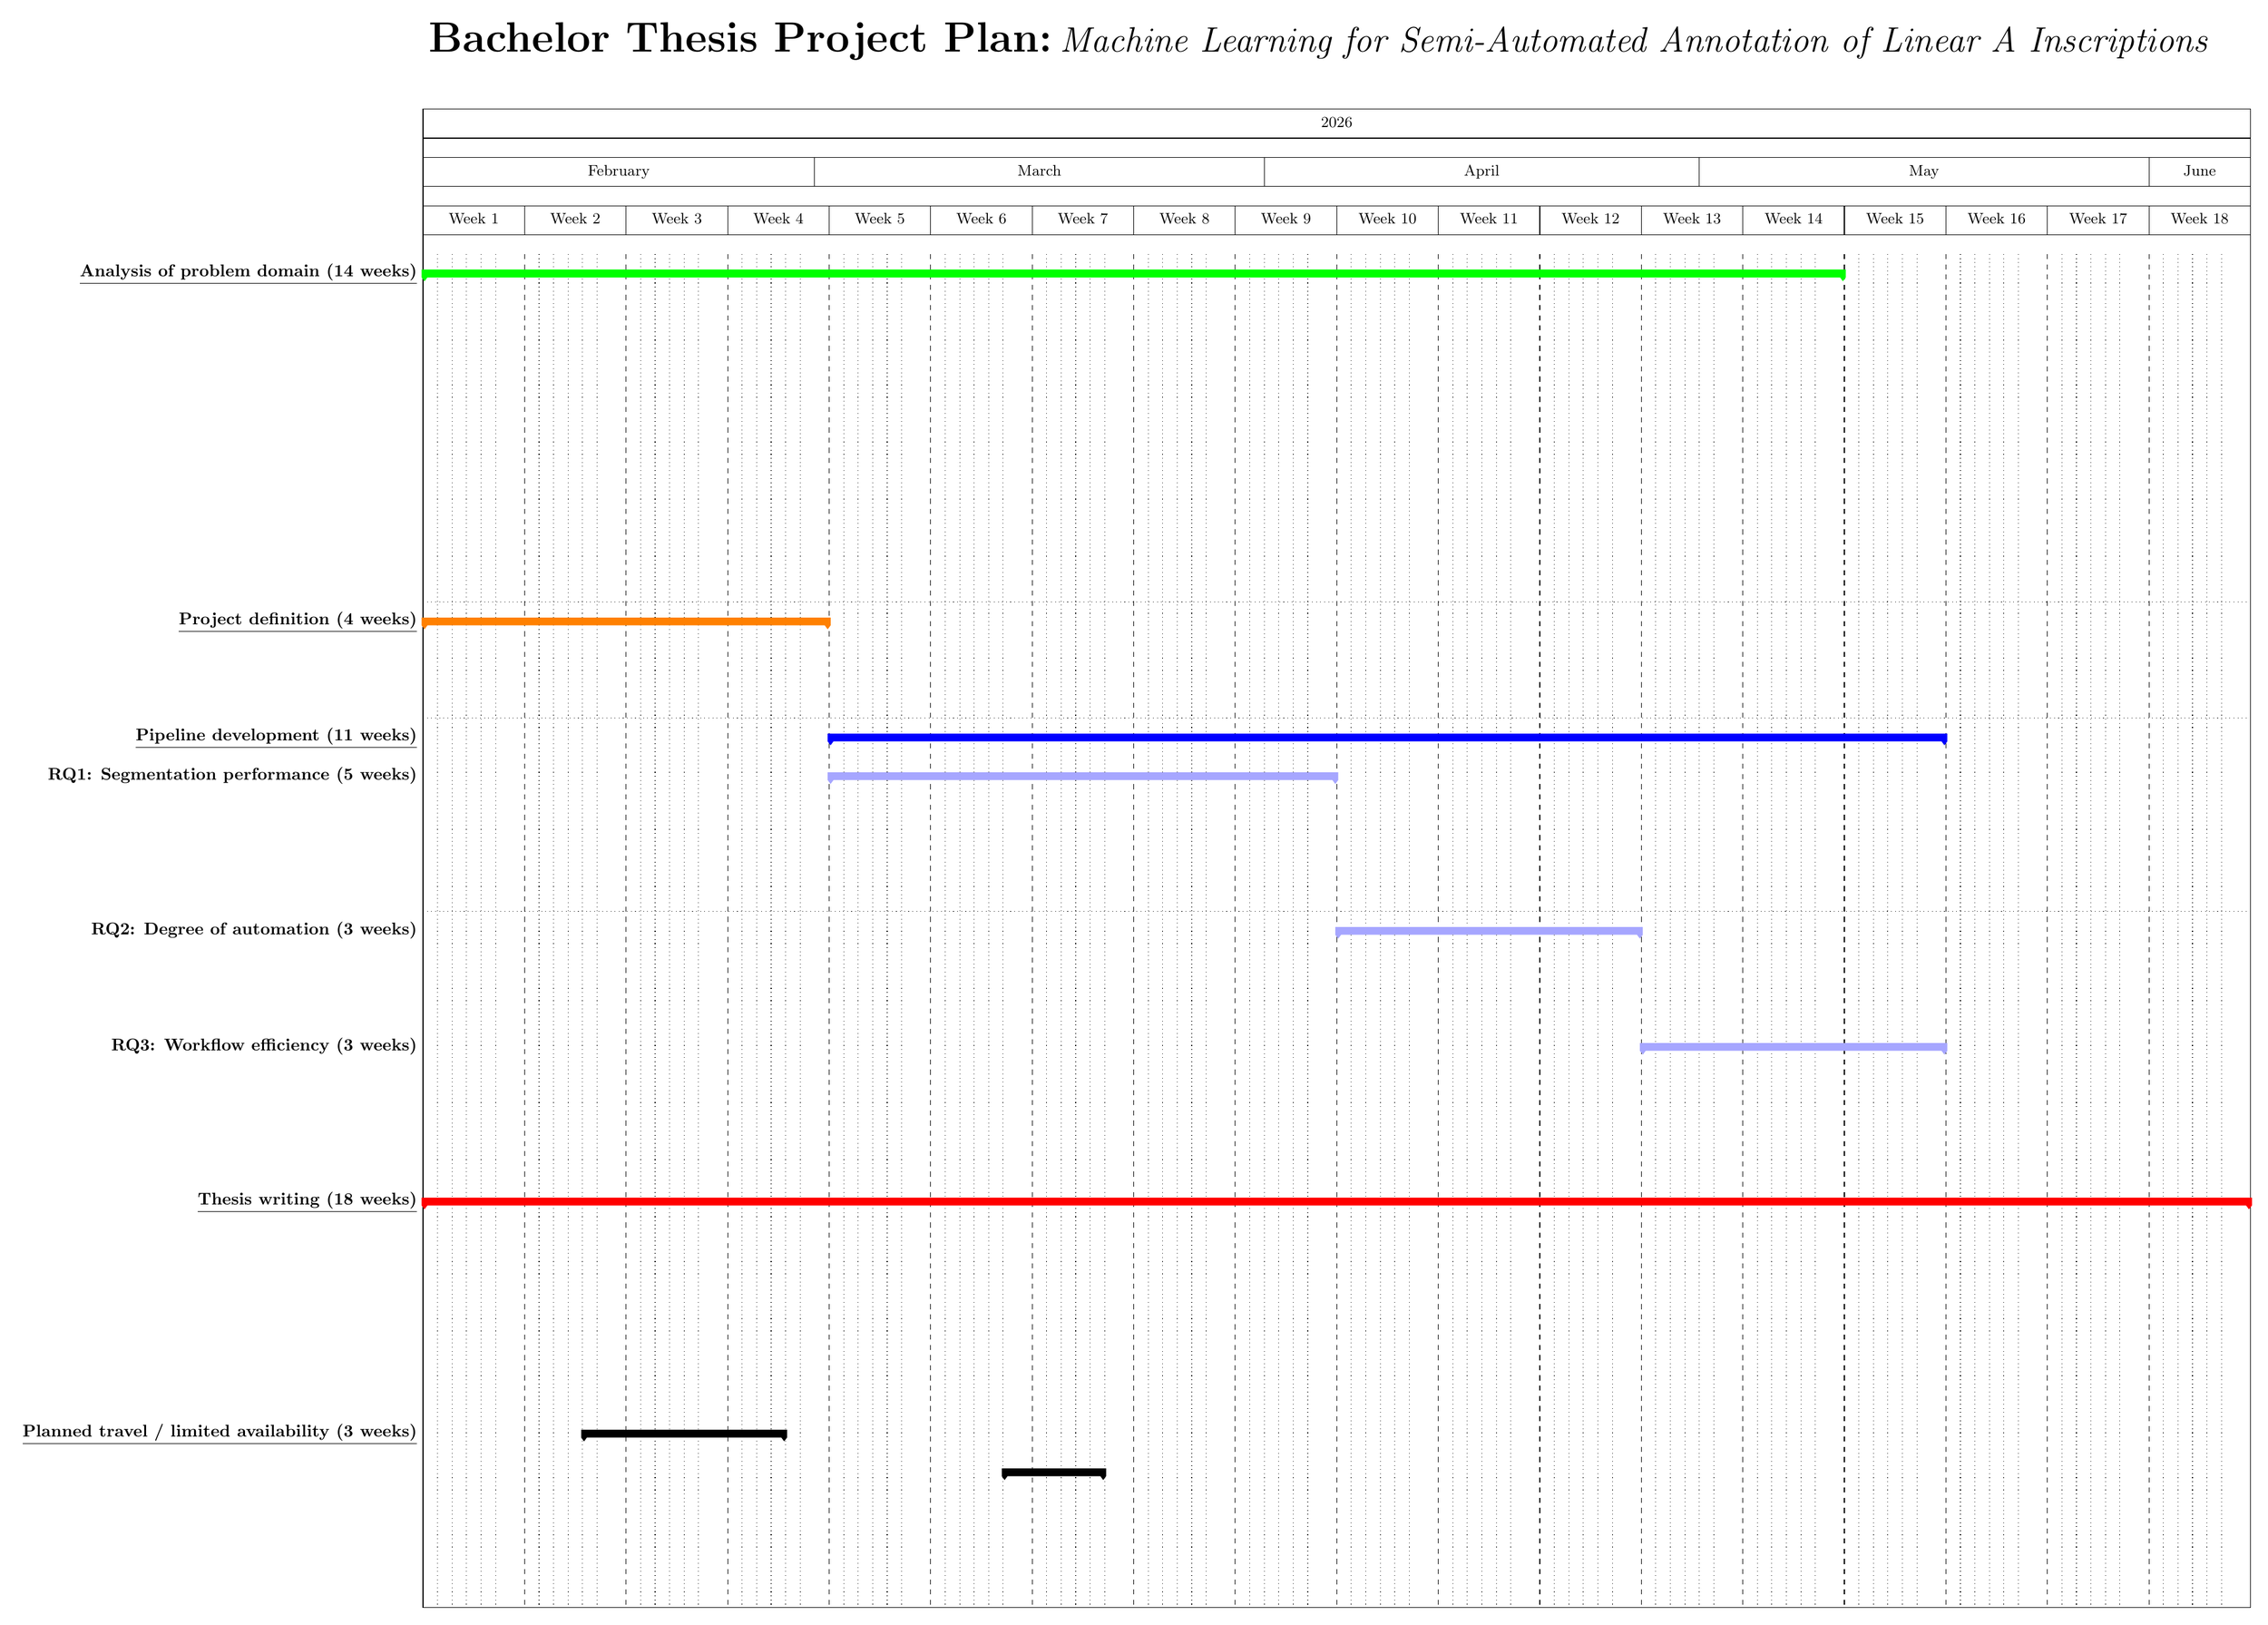
\begin{tikzpicture}
\node[anchor=west] at (0,1.4) {%
  {\Huge\bfseries Bachelor Thesis Project Plan:}\\[-0.2em]
  {\huge\itshape Machine Learning for Semi-Automated Annotation of Linear A Inscriptions}
};
\begin{ganttchart}[
  hgrid style/.style={black, dotted},
  vgrid={*5{black,dotted}, *1{white, dotted}, *1{black, dashed}},
  x unit=3mm,
  y unit chart=8mm,
  y unit title=10mm,
  time slot format=isodate,
  group label font=\bfseries,
  bar label font=\small,
  link/.style={->, thick}
]{2026-02-02}{2026-06-07}

\gantttitlecalendar{year, month=name, week}\\

% -------------------------
% Analysis of problem domain
% -------------------------
\ganttgroup[group/.append style={fill=green}]{\underline{Analysis of problem domain (14 weeks)}}{2026-02-02}{2026-05-10}\\
\ganttgreenbar[name=litreview]{Literature review (4 weeks)}{2026-02-02}{2026-03-01}\\
\ganttgreenbar[name=datacharacterization]{Data characterization (3 weeks)}{2026-03-02}{2026-03-22}\\
\ganttgreenbar[name=segmentation]{Segmentation + preprocessing review (4 weeks)}{2026-03-02}{2026-03-29}\\
\ganttgreenbar[name=groundtruth]{Ground truth + evaluation assessment (3 weeks)}{2026-03-16}{2026-04-05}\\
\ganttgreenbar[name=SAMprompt]{Study of SAM prompting behavior (2 weeks)}{2026-04-06}{2026-04-19}\\
\ganttgreenbar[name=clickexperimentdefinition]{Definition of interaction–quality evaluation (2 weeks)}{2026-04-13}{2026-04-26}\\
\ganttgreenbar[name=annotationworkflow]{Annotation workflow analysis (2 weeks)}{2026-04-27}{2026-05-10}\\
\ganttgreenbar[name=timestudyeval]{Definition of workflow efficiency evaluation (2 weeks)}{2026-04-27}{2026-05-10}\\[grid]

% -------------------------
% Project definition phase
% -------------------------
\ganttgroup[group/.append style={fill=orange}]{\underline{Project definition (4 weeks)}}{2026-02-02}{2026-03-01}\\
\ganttorangebar[name=pdr]{Project definition report (4 weeks)}{2026-02-02}{2026-03-01}\\
\ganttorangebar[name=gc]{Gantt chart (4 weeks)}{2026-02-02}{2026-03-01}\\[grid]


% -------------------------
% Implementation phase
% -------------------------
\ganttgroup[group/.append style={fill=blue}]{\underline{Pipeline development (11 weeks)}}{2026-03-02}{2026-05-17}\\
\ganttgroup[group/.append style={fill=blue!35}]{RQ1: Segmentation performance (5 weeks)}{2026-03-02}{2026-04-05}\\
\ganttbluebar[name=prep]{Image preprocessing (2 weeks)}{2026-03-02}{2026-03-15}\\
\ganttbluebar[name=sam]{SAM-based segmentation prototype (3 weeks)}{2026-03-09}{2026-03-29}\\
\ganttbluebar[name=export]{Ground truth extraction + evaluation metrics (3 weeks)}{2026-03-16}{2026-04-05}\\[grid]
\ganttgroup[group/.append style={fill=blue!35}]{RQ2: Degree of automation (3 weeks)}{2026-04-06}{2026-04-26}\\
\ganttbluebar[name=interactivity]{Interactive tooling with clicks (2 weeks)}{2026-04-06}{2026-04-19}\\
\ganttbluebar[name=clickexperiment]{Click-quality experiment + analysis (2 weeks)}{2026-04-13}{2026-04-26}\\
\ganttgroup[group/.append style={fill=blue!35}]{RQ3: Workflow efficiency (3 weeks)}{2026-04-27}{2026-05-17}\\
\ganttbluebar[name=stabilization]{Tool stabilization + SigLA-ready export (2 weeks)}{2026-04-27}{2026-05-10}\\
\ganttbluebar[name=timestudydesign]{Design of workflow eff. study [manual vs tool-assisted] (2 weeks)}{2026-04-27}{2026-05-10}\\
\ganttbluebar[name=timestudyexec]{Execution of workflow eff. study with Dr. Salgarella (1 week)}{2026-05-11}{2026-05-17}\\

% -------------------------
% Writing
% -------------------------
\ganttgroup[group/.append style={fill=red}]{\underline{Thesis writing (18 weeks)}}{2026-02-02}{2026-06-07}\\
\ganttredbar[name=intro]{Introduction Chapter (4 weeks)}{2026-02-02}{2026-03-01}\\
\ganttredbar[name=methdataimpl]{Method. + Data + Implement. Chapters (11 weeks)}{2026-03-02}{2026-05-17}\\
\ganttredbar[name=resultsdiscussion]{Results + Discussion Chapters (8 weeks)}{2026-03-30}{2026-05-24}\\
\ganttredbar[name=conclusion]{Conclusion Chapter + revision (3 weeks)}{2026-05-11}{2026-05-31}\\
\ganttredbar[name=final]{Final revision + thesis submission (2 weeks)}{2026-05-25}{2026-06-07}\\

% -------------------------
% Planned travel / limited availability
% -------------------------
\ganttgroup[
  group/.append style={fill=black}
]{\underline{Planned travel / limited availability (3 weeks)}}{2026-02-13}{2026-02-26}\\

\ganttgroup[
  group/.append style={fill=black},
  group label text={}
]{ }{2026-03-14}{2026-03-20}\\
\ganttblackbar[name=travel1]{Travel 1 (2 weeks)}{2026-02-13}{2026-02-26}\\
\ganttblackbar[name=travel2]{Travel 2 (1 week)}{2026-03-14}{2026-03-20}\\
% -------------------------
% Dependencies (these must reference existing names)
% -------------------------
%\ganttlink{pdr}{prep}



\end{ganttchart}

\end{tikzpicture}
\end{document}